%%%%%%%%%%%%%%%%%%%%%%%%%%%%%%%%%%%%%%%%%
% Beamer Presentation
% LaTeX Template
% Version 1.0 (10/11/12)
%
% This template has been downloaded from:
% http://www.LaTeXTemplates.com
%
% License:
% CC BY-NC-SA 3.0 (http://creativecommons.org/licenses/by-nc-sa/3.0/)
%
%%%%%%%%%%%%%%%%%%%%%%%%%%%%%%%%%%%%%%%%%

%----------------------------------------------------------------------------------------
%	PACKAGES AND THEMES
%----------------------------------------------------------------------------------------

\documentclass[aspectratio=169]{beamer}

\mode<presentation> {

 
% The Beamer class comes with a number of default slide themes
% which+++ change the colors and layouts of slides. Below this is a list
% of all the themes, uncomment each in turn to see what they look like.

%\usetheme{default}
%\usetheme{AnnArbor}
%\usetheme{Antibes}
%\usetheme{Bergen}
%\usetheme{Berkeley}
%\usetheme{Berlin}
%\usetheme{Boadilla}
%\usetheme{CambridgeUS}
%\usetheme{Copenhagen}
%\usetheme{Darmstadt}
%\usetheme{Dresden}
%\usetheme{Frankfurt}
%\usetheme{Goettingen}
%\usetheme{Hannover}
%\usetheme{Ilmenau}
%\usetheme{JuanLesPins}
%\usetheme{Luebeck}
\usetheme{Madrid}
%\usetheme{Malmoe}
%\usetheme{Marburg}
%\usetheme{Montpellier}
%\usetheme{PaloAlto}
%\usetheme{Pittsburgh}
%\usetheme{Rochester}
%\usetheme{Singapore}
%\usetheme{Szeged}
%\usetheme{Warsaw}

% As well as themes, the Beamer class has a number of color themes
% for any slide theme. Uncomment each of these in turn to see how it
% changes the colors of your current slide theme.

%\usecolortheme{albatross}
%\usecolortheme{beaver}
%\usecolortheme{beetle}
%\usecolortheme{crane}
%\usecolortheme{dolphin}
%\usecolortheme{dove}
%\usecolortheme{fly}
%\usecolortheme{lily}
%\usecolortheme{orchid}
%\usecolortheme{rose}
%\usecolortheme{seagull}
%\usecolortheme{seahorse}
%\usecolortheme{whale}
%\usecolortheme{wolverine}

%\setbeamertemplate{footline} % To remove the footer line in all slides uncomment this line
%\setbeamertemplate{footline}[page number] % To replace the footer line in all slides with a simple slide count uncomment this line

\definecolor{UOSred}{rgb}{0.6745098039215686, 0.02352941176470588, 0.2039215686274510} % UBC Blue (primary)
\definecolor{UOSgrey}{rgb}{0.8117647058823529, 0.8117647058823529, 0.8117647058823529} % UBC Grey (secondary)

\setbeamercolor{palette primary}{bg=UOSred,fg=white}
\setbeamercolor{palette secondary}{bg=UOSred,fg=white}
\setbeamercolor{palette tertiary}{bg=UOSred,fg=white}
\setbeamercolor{palette quaternary}{bg=UOSred,fg=white}
\setbeamercolor{structure}{fg=UOSred} % itemize, enumerate, etc
\setbeamercolor{section in toc}{fg=UOSred} % TOC sections

%gets rid of bottom navigation bars
\setbeamertemplate{footline}[frame number]{}

%gets rid of bottom navigation symbols
\setbeamertemplate{navigation symbols}{}


\usepackage{amsmath}
\usepackage{selinput}      % Halbautomatische Auswahl der Eingabecodierung
\SelectInputMappings{      % mit Hilfe ausgewählter Glyphen
  adieresis={ä},	   % siehe: http://partners.adobe.com/public/developer/en/opentype/glyphlist.txt
  germandbls={ß},
  Euro={€}
}

\addtobeamertemplate{footline}{%
  \leavevmode%
  \hbox{%
  \begin{beamercolorbox}[wd=\paperwidth,ht=2.25ex,dp=1ex,center]{author in head/foot}%
     \insertsectionnavigationhorizontal{\paperwidth}{}{}
  \end{beamercolorbox}}%

}

% Override palette coloring with secondary
\setbeamercolor{subsection in head/foot}{bg=UOSgrey,fg=white}

%\setbeamertemplate{navigation symbols}{} % To remove the navigation symbols from the bottom of all slides uncomment this line
}
\usepackage{hyperref}
\usepackage{graphicx} % Allows including images
\usepackage{grffile}
\usepackage{booktabs} % Allows the use of \toprule, \midrule and \bottomrule in tables
\graphicspath{{images/}}

% ------------------------------------------------------------------------------------------------------------------------------------------------

\title[ScheduleMe]{ScheduleMe - Phase 2}

\author{T. Adam, M. ben Ahmed, M. Hündorf, D. Massanés}
\institute[UOS]
{

Universität Osnabrück \\ % Your institution for the title page

\medskip
\textit{Ressourcenbeschränkte Projektplanung} % Your email address


}
\date{\today} % Date, can be changed to a custom date

\begin{document}

\begin{frame}
\titlepage % Print the title page as the first slide
\end{frame}

% ------------------------------------------------------------------------------------------------------------------------------------------------

\begin{frame}
	\frametitle{ScheduleMe - Überblick}
	\begin{columns}[c] % The "c" option specifies centered vertical alignment while the "t" option is used for top vertical alignment
		
		\column{.55\textwidth} % Left column and width
		\textbf{Projektstruktur}
		\begin{itemize}
			\item Implementiert in C++
			\item Earliest Start Schedule
			\item Simulated Annealing
		\end{itemize}
		\column{.35\textwidth} % Left column and width
		
\includegraphics[scale=.5]{../images/stock.jpg}
	\end{columns}
\end{frame}
  
% ------------------------------------------------------------------------------------------------------------------------------------------------
	
\begin{frame}[t]
\frametitle{ScheduleMe - Optimierungen}

	\vspace{-8pt}
	\textbf{Allgemein}
	\begin{itemize}
		\item Arrayzugriff ohne Überprüfung der Grenzen
		\item Beseitigung redundanter und verzichtbarer Operationen
		\item Automatische Compileroptimierung
	\end{itemize}

	\vspace{6pt}
	\textbf{Simulated Annealing}
	\begin{itemize}
		\item Dynamische Updates des Abkühlungsfaktors
	\end{itemize}

	\vspace{6pt}
	\textbf{Earliest Start Schedule}
	\begin{itemize}
		\item Sprungstellen
	\end{itemize}

	\vspace{6pt}
	\textbf{Nachbarschaften}
	\begin{itemize}
		\item $\mathcal{N}_{api}$ optimiert
		\item Binäre Suche
	\end{itemize}

\end{frame}

% ------------------------------------------------------------------------------------------------------------------------------------------------

\begin{frame}
	\frametitle{ScheduleMe - Profiler, alter Stand}
	
		\vspace{-6pt}
	
		\begin{figure}
			\centering
			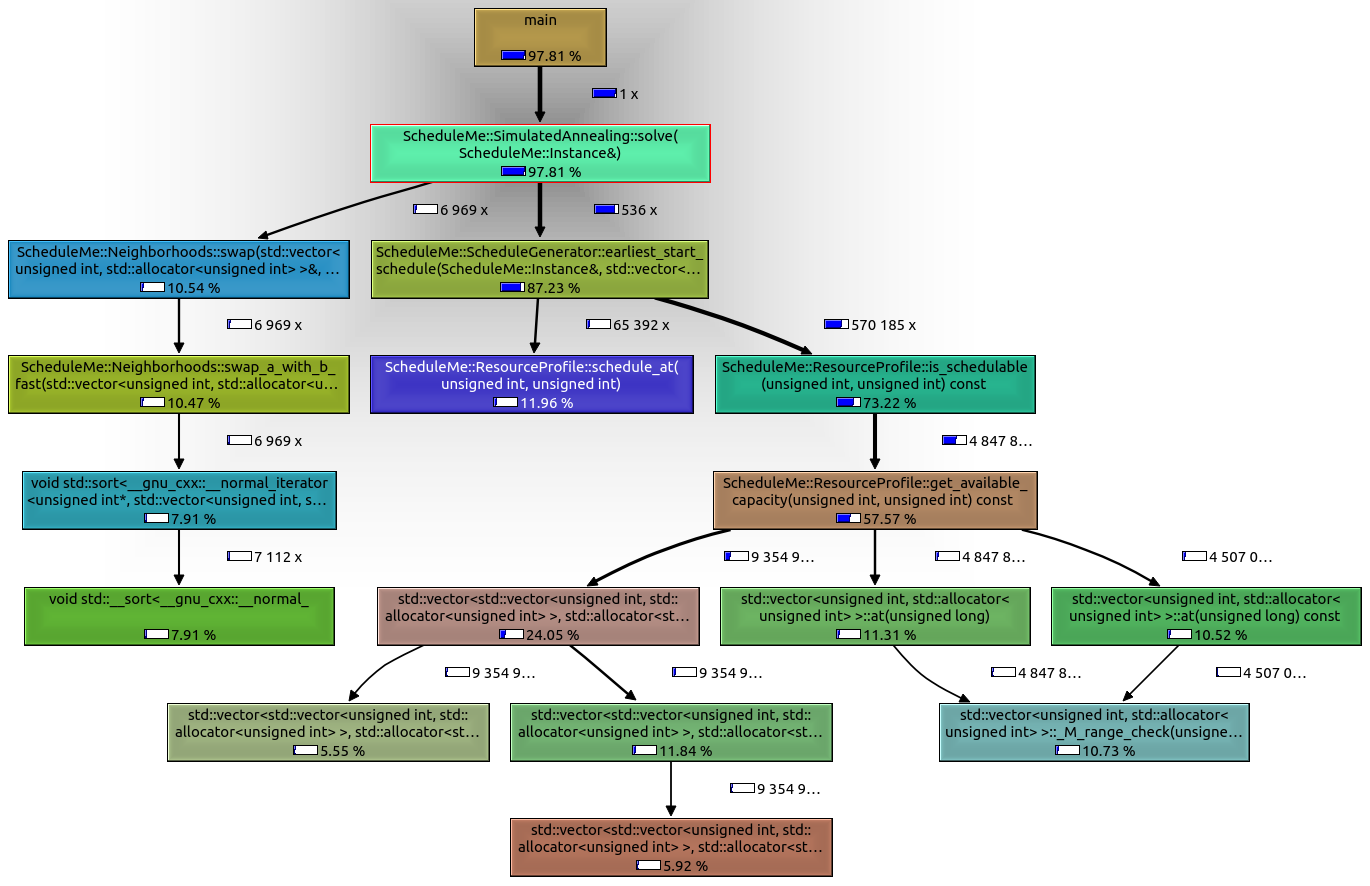
\includegraphics[scale=0.237]{profiler_old_O0_full.png}
		\end{figure}
	
	\end{frame}
	
% ------------------------------------------------------------------------------------------------------------------------------------------------

\begin{frame}
\frametitle{ScheduleMe - Profiler, Vergleich mit Compileroptimierung}

	\begin{columns}[c]
		\column{.39\textwidth}
			\centering
			\vspace{10pt}
			\textbf{Alter Stand}
			
\includegraphics[width=\textwidth]{../images/profiler_old_O3.png}
		\column{.6\textwidth}
			\centering
			\vspace{10pt}
			\textbf{Neuer Stand}
		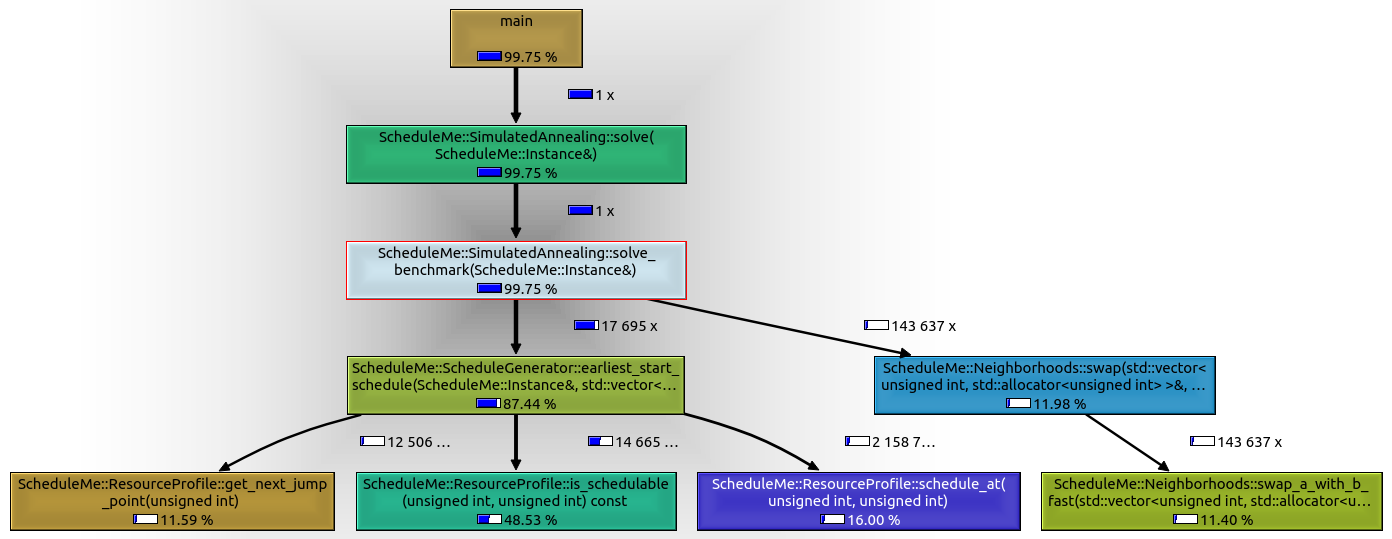
\includegraphics[width=\textwidth]{../images/profiler_new_O3.png}
	\end{columns}

\end{frame}

% ------------------------------------------------------------------------------------------------------------------------------------------------

\begin{frame}
\frametitle{ScheduleMe - Vergleich Implementierungen}
	
	\begin{columns}[c]
		\column{.33\textwidth}
			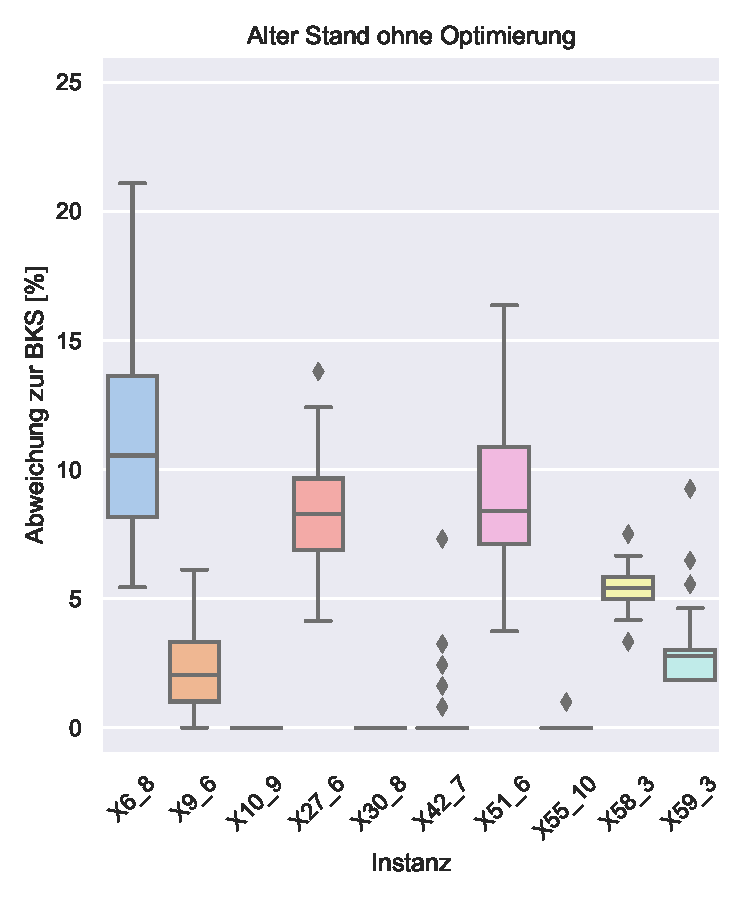
\includegraphics[width=\textwidth]{../images/results_old.pdf}	
		\column{.33\textwidth}
			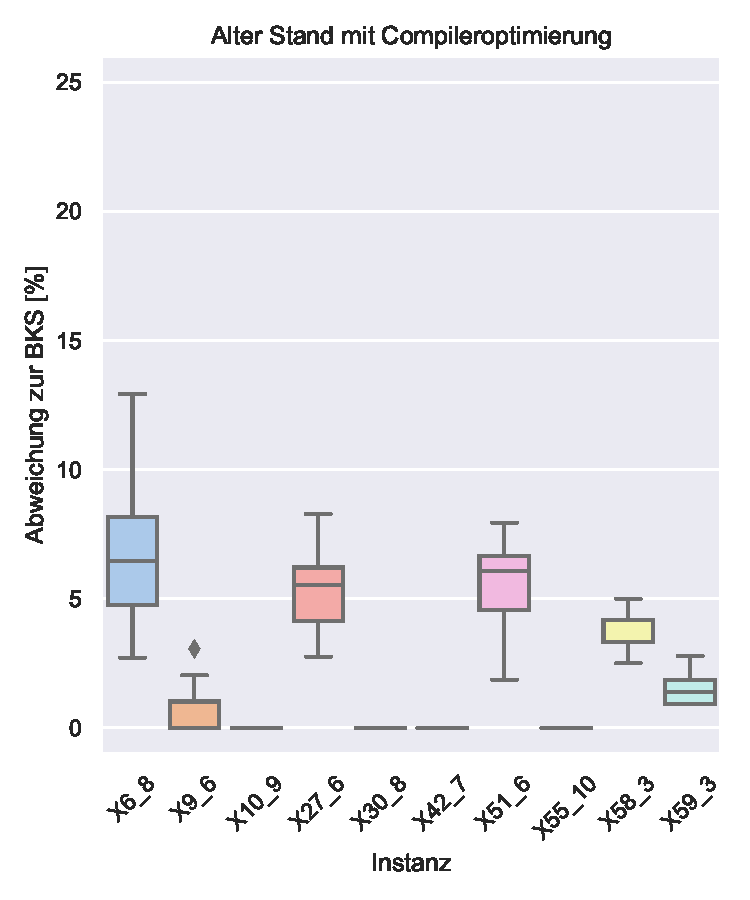
\includegraphics[width=\textwidth]{../images/results_oldo3.pdf}	
		\column{.33\textwidth}
			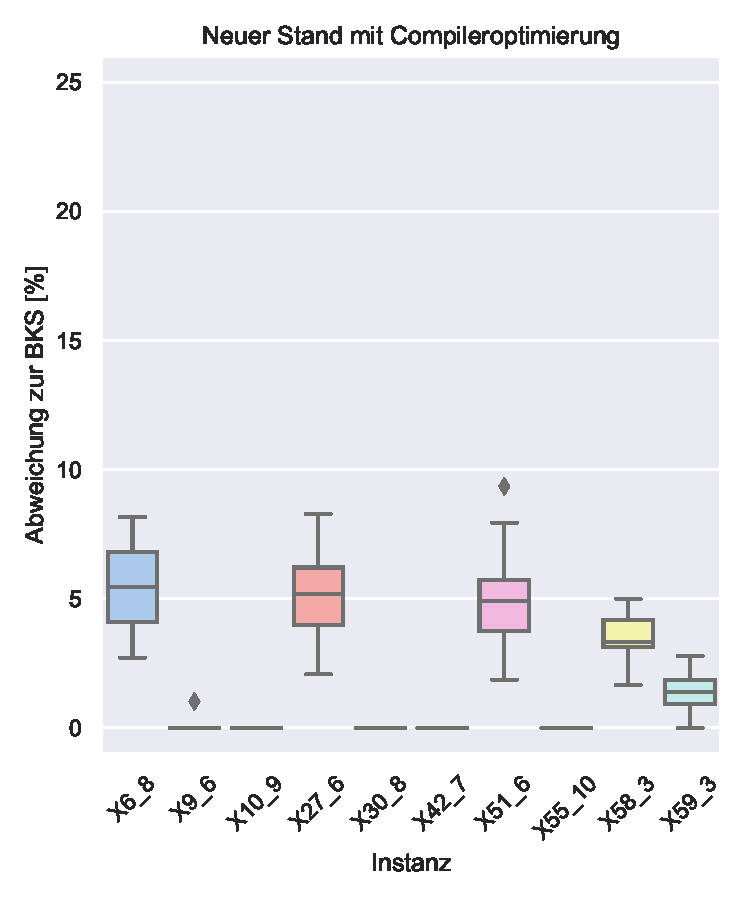
\includegraphics[width=\textwidth]{../images/results_new.pdf}	
	\end{columns}

\end{frame}
	
% ------------------------------------------------------------------------------------------------------------------------------------------------

\begin{frame}
\frametitle{ScheduleMe - Vergleich Nachbarschaften}

	\vspace{-6pt}

	\begin{figure}
		\centering
		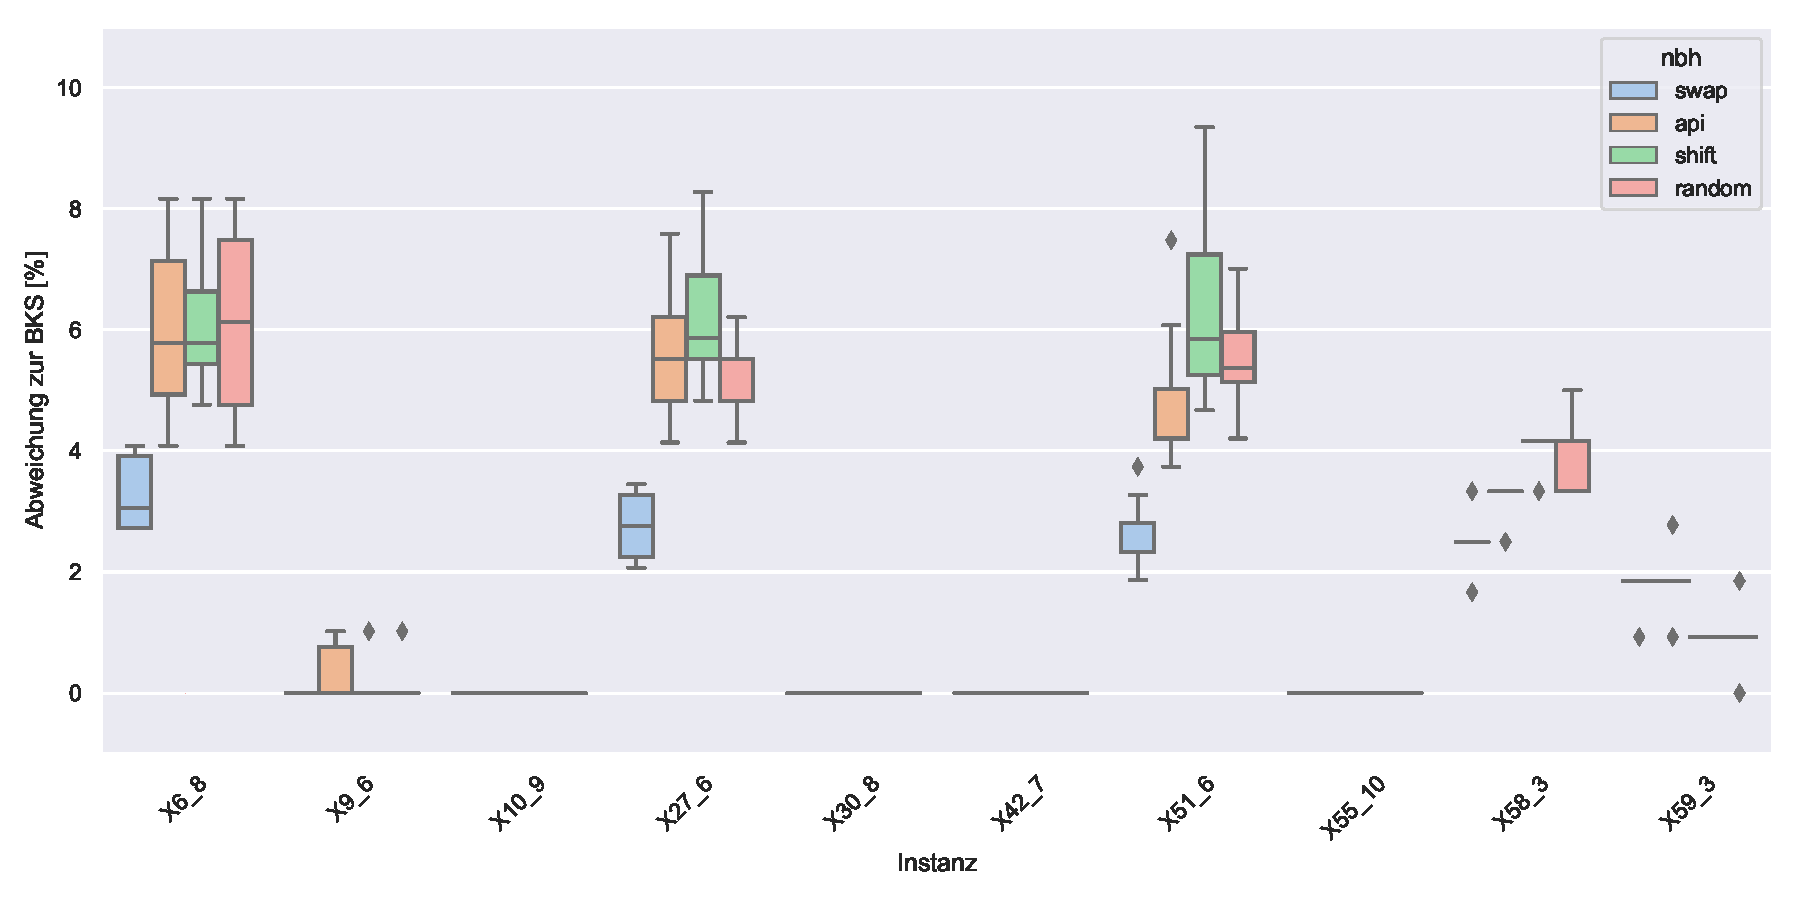
\includegraphics[height=0.9\textheight]{../images/results_nbhs.pdf}
	\end{figure}
	
\end{frame}

\end{document}

